\documentclass[11pt,a4paper]{article}
\usepackage[utf8]{inputenc}
\usepackage{amsmath}
\usepackage{amsfonts}
\usepackage{amssymb}
\usepackage[pdftex]{graphicx}
\usepackage{float}
\setlength{\parindent}{0in}
\begin{document}
\tableofcontents
\newpage

\section{Vision}
\subsection{Introduction}
Our goal is to make an interactive document sharing system, Slice of Pie,  which allows multiple users to easily share and edit documents both online and offline.
\subsection{Problem statement}
Sharing and editing documents can be cumbersome. \\
Sending a document back and forth between multiple users can lead to a lot of errors. Users can overwrite what another user has done, and if they aren't all using the same text editing system this can lead to formatting issues in the document.
\subsection{Summary of system features}
\begin{enumerate}
\item Multiple users must be able to share and edit documents online.
\item Synchronization for offline usage.
\item Merging of documents.
\item History. Which allows the user to see all recent changes made to the document.
\item Documents can be categorized into folders or projects in order to get a better overview when working on a larger project with multiple files.
\end{enumerate}

\section{Use cases}
\begin{enumerate}
\item UC1: Create new document
\item UC2: Edit document
\item UC3: Delete document
\item UC4: Merging documents (resolve conflict)
\item UC5: Offline sync
\item UC6: New folder
\item UC7: New project
\item UC8: Find old version of document
\item UC9: Share Document
\item UC10: Log in
\end{enumerate}

% Use case 1
\fbox{\begin{minipage}{\columnwidth}
		\textbf{Use case UC1: Create new document} \\ 
		\textbf{Scope:} Slice-of-pie application \\
		\textbf{Level:} User goal \\
		\textbf{Primary actor:} Regular user \\
		\textbf{Stakeholders and Interests: } \\
		- Regular user: Wants to create a new document without any complications. \\
		\textbf{Preconditions:} none. \\
		\textbf{Postconditions:} The document will be created\\
		
		\textbf{Basic flow:} 
		\begin{enumerate}
			\item The user needs a document that can be shared with others.
			\item The user chooses a client program (web or desktop client).
			\item The user presses the "New Document" button.
			\item The client presents a dialogue box.
			\item The user types information about the document and press OK.
			\item The client sends a request to the server and the document gets stored by the server.
			\item The client displays the document for the user.
		\end{enumerate} 
		\textbf{Extensions:}
			\begin{enumerate}
				\item[6.]  The server is not responding \\
				\begin{enumerate}
					\item The document is saved locally.
					\item The client requests the server in regular intervals to see if it has recovered.
				\end{enumerate}
			\end{enumerate}
		\textbf{Special requirements:} \\
		- The document should be displayed properly on any devices such as smart phones and tablets. \\
\end{minipage}}

% Use case 2
\fbox{\begin{minipage}{\columnwidth}
		\textbf{Use case UC2: Edit document} \\ 
		\textbf{Scope:} Slice-of-pie application \\
		\textbf{Level:} User goal \\
		\textbf{Primary actor:} Regular user \\
		\textbf{Preconditions:} A document must have been created \\
		\textbf{Postconditions:} The document must be edited the way the user desires and the change must be recorded by the server too\\
		
		\textbf{Basic flow:} 
		\begin{enumerate}
			\item The user opens a document.
			\item The user edits the content of the document.
			\item The client sends a request to the server.
			\item The document is changed on the server.
		\end{enumerate} 
		\textbf{Extensions:}
			\begin{enumerate}
				\item[3.]  The server is not responding \\
				\begin{enumerate}
					\item The document is saved locally.
					\item The client requests the server in regular intervals to see if it has recovered.
				\end{enumerate}
			\end{enumerate}
		\textbf{Special requirements:} \\
		- The document should be displayed properly on any devices such as smart phones and tablets. \\		
\end{minipage}}

% Use case 3
\fbox{\begin{minipage}{\columnwidth}
		\textbf{Use case UC3: Delete document } \\ 
		\textbf{Scope:} Slice-of-pie application \\
		\textbf{Level:} User goal \\
		\textbf{Primary actor:} Regular user \\
		\textbf{Preconditions:} A document must have been created. The user trying to delete a document must have sufficient rights to delete selected document \\
		\textbf{Postconditions:} The document is now deleted from the users local repository, and will be deleted when user commits \\
		
		\textbf{Basic flow:} 
			\begin{enumerate}
			\item The user selects a document
			\item The user tries to delete the document 3. The client sends a request to the server 
			\item Server checks for authentication
			\item Document is deleted
			\end{enumerate}
		\textbf{Extensions:}
			\begin{enumerate}
			\item[3.] The server is not responding
			\begin{itemize}
			\item The document is saved locally
			\item The client requests the server in regular intervals to see if it has recovered			
			\end{itemize}
			\item[4.] The user lacks the right to delete the selected document
			\begin{itemize}
			\item User is told that he has not got the rights to delete selected document
			\end{itemize} 
			\end{enumerate}
		\textbf{Special requirements:} \\
\end{minipage}}	

% Use case 4
\fbox{\begin{minipage}{\columnwidth}
		\textbf{Use case UC4: Merging documents (Resolve conflict)} \\ 
		\textbf{Scope:} Slice of Pie application\\
		\textbf{Level:}  User goal\\
		\textbf{Primary actor:} Regular user\\
		\textbf{Preconditions:} A document must exist on the server and another (edited) version of the same document must exist on the stand-alone client\\
		\textbf{Postconditions:} Both versions (client and server) must have matching content\\
		
		\textbf{Basic flow:} 
		\begin{enumerate}
		\item The user opens an existing document on the client.
		\item The user edits the document and saves the lates changes.
		\item The stand-alone client and the server are synchronized.
		\item Both documents merge and contain both the original and the new content.
		\end{enumerate}
		\textbf{Extensions:} 
		\begin{enumerate}
		\item[*4.] There is a conflict when merging the documents.
		\begin{enumerate}
		\item The user resolves the conflict manually by editing the document.
		\item The user synchronizes again.
		\end{enumerate}				
		\end{enumerate}
		\textbf{Special requirements:} \\
\end{minipage}}

% Use case 5
\fbox{\begin{minipage}{\columnwidth}
		\textbf{Use case UC5: Offline synchronization} \\ 
		\textbf{Scope:} Slice-of-pie application \\
		\textbf{Level:} User goal \\
		\textbf{Primary actor:} Regular user \\
		\textbf{Preconditions:} User must be logged in. Client must be connected to the server. \\
		\textbf{Postconditions:} The users offline repository will be synchronized with his online repository \\
		
		\textbf{Basic flow:} \\
		\begin{enumerate}
		\item The user selects offline synchronization
		\item The client sends a request to the server.
		\item The server copies the user's online repository and sends it to the client
		\item The client sends verification upon receiving the documents
		\end{enumerate}
		\textbf{Extensions:} \\
		\begin{enumerate}
		\item[2.] The server is not responding
			\begin{itemize}
			\item The user gets an error message (no connection)
			\end{itemize}
		\item[4.] The server is not responding
			\begin{itemize}
			\item The client tries to re-establish a connection to the server at regular intervals, and then sends the verification.
			\end{itemize}
		\end{enumerate}
		\textbf{Special requirements:} \\
\end{minipage}}

% Use case 6
\fbox{\begin{minipage}{\columnwidth}
		\textbf{Use case UC6: Create new folder} \\ 
		\textbf{Scope:} Slice-of-pie application\\
		\textbf{Level:} User goal\\
		\textbf{Primary actor:} Regular user\\
		\textbf{Preconditions:} none.\\
		\textbf{Postconditions:} The folder will have been created\\
		
		\textbf{Basic flow:} 
		\begin{enumerate}
			\item User clicks on "create new folder" button
			\item User fills in valid folder information and clicks "OK"
			\item Client sends a request to server and server stores the folder
			\item Client displays the new folder
		\end{enumerate}
		\textbf{Extensions:} 
		\begin{enumerate}
			\item[2.] Information is not valid
			\begin{enumerate}
				\item User gets an error message describing what information is invalid
			\end{enumerate}
			\item[3.] Server does not respond
			\begin{enumerate}
				\item folder is stored locally
				\item The client requests the server in regular intervals to see if it has recovered, then resends the request to create a folder.
			\end{enumerate}
		\end{enumerate}
		\textbf{Special requirements:} \\
\end{minipage}}

% Use case 7
\fbox{\begin{minipage}{\columnwidth}
		\textbf{Use case UC7: Create new project} \\ 
		\textbf{Scope:} Slice-of-pie application\\
		\textbf{Level:}  User goal\\
		\textbf{Primary actor:} Regular user\\
		\textbf{Preconditions:} none.\\
		\textbf{Postconditions:} a Project will have been created\\
		
		\textbf{Basic flow:} \begin{enumerate}
			\item User clicks on "Create New Project" button
			\item User fills in valid Project information and clicks "OK"
			\item Client sends a request to server and server stores the Project
			\item Client displays the new folder
		\end{enumerate}
		\textbf{Extensions:} 
		\begin{enumerate}
			\item[2.] Information is not valid
			\begin{enumerate}
				\item User gets an error message describing what information is invalid
			\end{enumerate}
			\item[3.] Server does not respond
			\begin{enumerate}
				\item Project is stored locally
				\item The client requests the server in regular intervals to see if it has recovered, then resends the request to create a Project.
			\end{enumerate}
		\end{enumerate}
		\textbf{Special requirements:} \\
\end{minipage}}

% Use case 8
\fbox{\begin{minipage}{\columnwidth}
		\textbf{Use case UC8: View old version of document} \\ 
		\textbf{Scope:} Slice of Pie application\\
		\textbf{Level:} User goal\\
		\textbf{Primary actor:} Regular user \\
		\textbf{Preconditions:} A document with multiple changes must exist \\
		\textbf{Postconditions:} None\\		
		\textbf{Basic flow:} 
		\begin{enumerate}
		\item A user wants to see an overview of all changes made to a document.
		\item User opens a document.
		\item User presses a button and is presented with a list of all changes made to the specific document.
		\end{enumerate}
		\textbf{Extensions:} \\
		\textbf{Special requirements:} \\
\end{minipage}}

% Use case 9
\fbox{\begin{minipage}{\columnwidth}
		\textbf{Use case UC9:} Share document \\
		\textbf{Scope:} Slice of Pie application \\
		\textbf{Level:}  User goal\\
		\textbf{Primary actor:} Regular user\\
		\textbf{Preconditions:} A document must be created in the system and at least two users must be registered.\\
		\textbf{Postconditions:} The document is shared between two (or more) users.\\
		
		\textbf{Basic flow:} 
		\begin{enumerate}
		\item The users creates a new document or opens an existing one.
		\item The user selects which users he wants to share the document with.
		\item The user shares the document with the selected user(s).
		\end{enumerate}
		\textbf{Extensions:} \\
		\textbf{Special requirements:} \\
\end{minipage}}

% Use case 10
\fbox{\begin{minipage}{\columnwidth}
		\textbf{Use case UC10: Log in} \\ 
		\textbf{Scope:} Slice of Pie application\\
		\textbf{Level:}  User goal\\
		\textbf{Primary actor:} Regular user\\
		\textbf{Preconditions:} User must be registered in the system \emph{(see "extensions *2").}\\
		\textbf{Postconditions:} User is logged into the system.\\
		
		\textbf{Basic flow:} \\
		\begin{enumerate}
			\item When the user starts the system (web client or stand-alone client) he's prompted with a login screen.
			\item User must log in by typing username and password.
			\item System checks if information matches what is stored in the system.
			\item User is logged into the system.
		\end{enumerate}
		\textbf{Extensions:} \\
		\begin{enumerate}
			\item[*2.] User is not registered in the system.
		\begin{enumerate}
			\item User is prompted with a sign up screen (web-client only).
			\item User fills out required information for signing up.
		\end{enumerate}
			\item[*4.] Username and password are rejected.
		\begin{enumerate}
			\item User gets an error message on the screen saying that the username and password don't match the system.
			\item User gets prompted back to the login screen.
		\end{enumerate}
		\end{enumerate}
		\textbf{Special requirements:} \\
\end{minipage}}

\section{Glossary}
\begin{itemize}
\item \textbf{Response Time:} The time it takes for the system to respond to a request from the user.
\item \textbf{Document:} A document refers to a complete document, not just a single file. A document contains a owner, id, content and a file.
\item \textbf{Client:} A client can mean two things. A web client, operating directly on the server, and a stand-alone client, that runs offline, locally on the end users machine synchronizing with the server.
\item \textbf{System:} Refers to the core of the application. This includes document handler, user handler etc ..
\end{itemize}

\section{Supplementary Specification (FURPS+)}
\begin{itemize}
\item Functionality
	\begin{itemize}
	\item The system must be able to create/edit/delete users.
    \item The system must be able to create/edit/delete/share documents.
    \item The system must keep a log of all document actions.
    \item All system usage requires user authentication.
	\item The system must support multiple users.
	\end{itemize}
\item Usability
	\begin{itemize}
    \item The system must be easy to use.
    \begin{itemize}
	\item Have a clean user interface.
    \item 8 out of 10 users must be able to use the system without any training.    
    \end{itemize}
    \item The system must be easily visible for people with "not perfect" vision. 
     E.g no graphics that blurs the view of the core system functionality.
    \item The web client must be easy and quick to navigate. No function should 
     be more than 3 clicks (windows/sub-windows) away.
     \begin{itemize}
     \item Not counting navigating a users files.     
     \end{itemize}
	\end{itemize}
\item Reliability
	\begin{itemize}
	\item It must be possible to use the system without any internet connection.
	\begin{itemize}
	\item With some limitations.
	\end{itemize}
	\end{itemize}
\item Performance
	\begin{itemize}
    \item The system must respond instantly
    \begin{itemize}
	 \item A request must not take more than a few (2-3) seconds.
     \item Not taking external factors (such as bad internet connection) into account.    
    \end{itemize}
	\end{itemize}
\end{itemize}

\section{Domain Model}
	\begin{figure}[h]
  		\centering
    	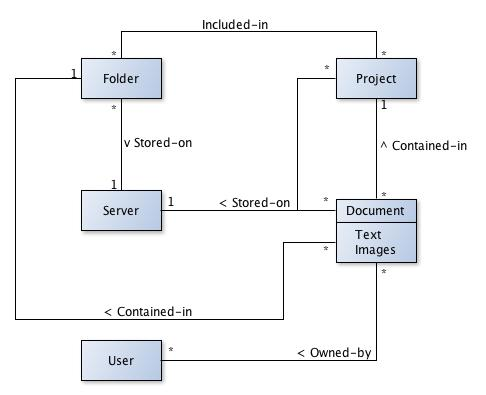
\includegraphics[width=300px]{images/DomainModel.jpg}
    	\caption{Domain Model}
	\end{figure}
	
\section{Logical Architecture}
	\begin{figure}[H]
  		\centering
    	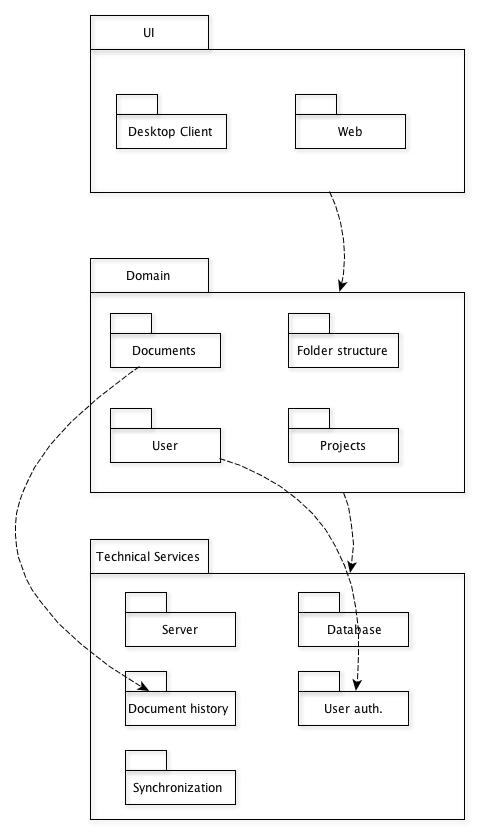
\includegraphics[width=300px]{images/LogicalArchitecture.jpg}
    	\caption{Logical Architecture}
	\end{figure}

\section{System Sequence Diagram}
	\begin{figure}[H]
  		\centering
    	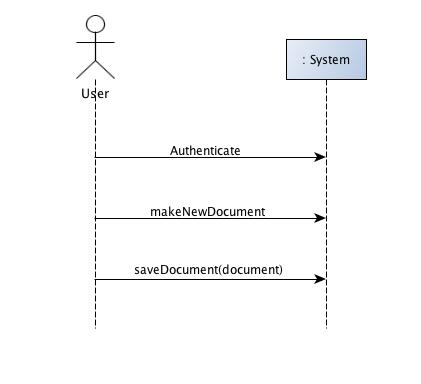
\includegraphics[width=300px]{images/SSQ_NewDocument.jpg}
    	\caption{SSD - New document}
	\end{figure}
	
\section{Operation Contracts}
\fbox{\begin{minipage}{\columnwidth}
		\textbf{Contract CO1:} Synchronize \\ 
		\textbf{Operation:} Synchronize \\
		\textbf{Cross References:} UC1, UC2, UC5 \\
		\textbf{Preconditions:} Some documents and/or must have been created on the system. \\
		\textbf{Postconditions:} \\
		 - All documents and folders on the client must be uploaded to the server. \\
		- All documents and folders on the server must be downloaded to the client. \\
		- Document version must be the same on the client and server.
\end{minipage}}

\section{Use Case Diagram}
	\begin{figure}[H]
  		\centering
    	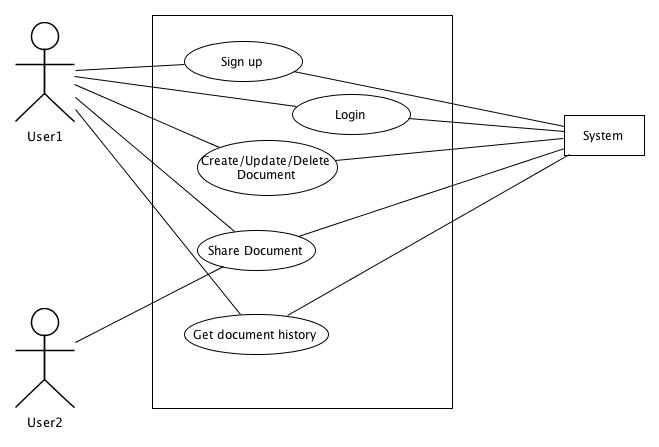
\includegraphics[width=300px]{images/UpdatedUsecaseDiagram.jpg}
    	\caption{Use case diagram}
	\end{figure}

\section{UML Package Diagram}
	\begin{figure}[H]
  		\centering
    	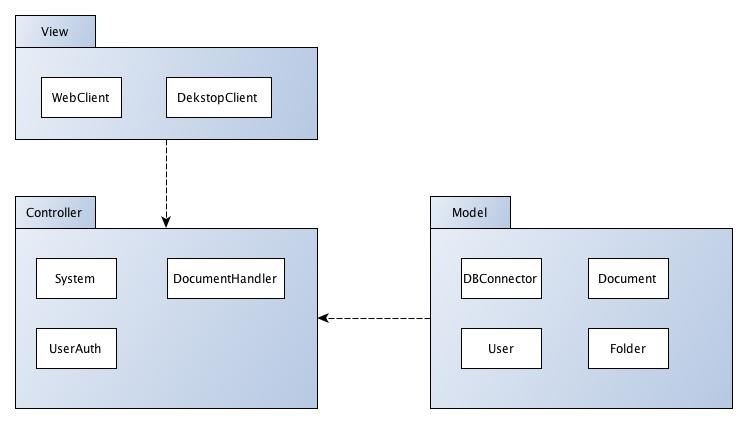
\includegraphics[width=300px]{images/PackageDiagramOverview.jpg}
    	\caption{Package Diagram Overview}
	\end{figure}

\section{UML Class Diagram}
	\begin{figure}[H]
  		\centering
    	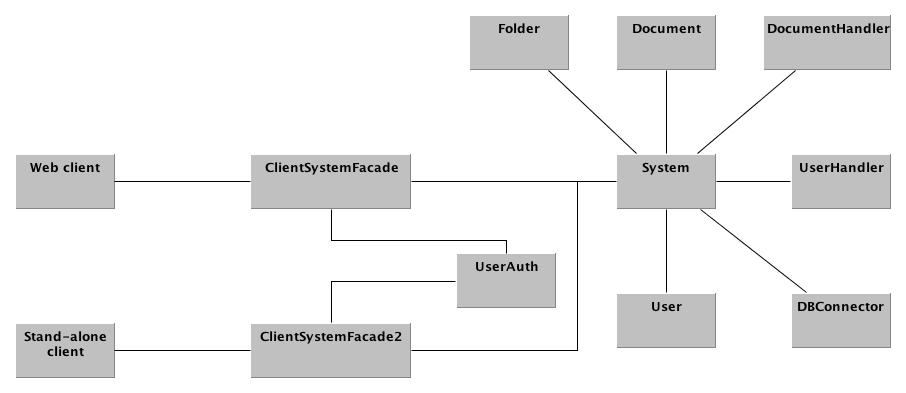
\includegraphics[width=300px]{images/LatestClassDiagram.jpg}
    	\caption{Class Diagram Overview}
	\end{figure}
	
\section{Communication Diagram}
	\begin{figure}[H]
  		\centering
    	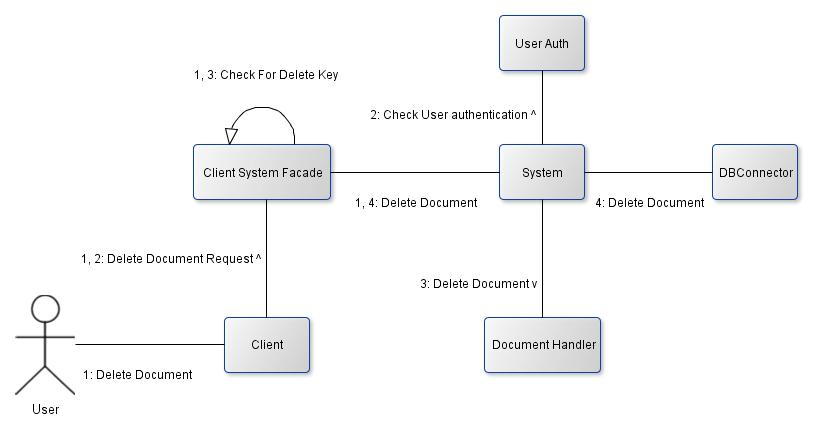
\includegraphics[width=300px]{images/Communication Diagrams/Delete Communication Diagram.jpg}
    	\caption{Communication Diagram}
	\end{figure}

\section{Technical Memo}
	\fbox{\begin{minipage}{\columnwidth}
	\begin{center}
		\textbf{Technical Memo} \\
		\textbf{Issue: Files format - Which file format to use}
	\end{center}
	\textbf{Solution Summary:} Use HTML for our file format.\\
	\textbf{Factors}
		\begin{itemize}
			\item Must be able to contain both text and images.
		\end{itemize}
	\textbf{Solution} \\
	We chose to use HTML for our file format because it's simple to construct, and can contain text and images seamlessly. \\
	\textbf{Motivation} \\
	We needed a file format that can contain images and text as well as being easy to construct. in addition, HTML can easily be extended to other content. Lastly, HTML can be opened with any browser, so the users isn't tied to SliceOfPie if he just want's to view the content of a file. \\
	\textbf{Alternatives considered} \\
	We considered using a .txt file format, but .txt can only contain plain text. \\
	We also considered using our own file format (since the format itself isn't important to the application). But if we use our own format the user is stuck with using SliceOfPie, so he can't view the content of a file with any other application.
\end{minipage}}

\fbox{\begin{minipage}{\columnwidth}
	\begin{center}
		\textbf{Technical Memo} \\
		\textbf{Issue: Merging two versions of the same document.}
	\end{center}
	\textbf{Solution Summary:} Git-hub inspired merge.\\
	\textbf{Factors}
		\begin{itemize}
			\item Merging two versions of the same document without overwriting existing changes.
		\end{itemize}
	\textbf{Solution} \\
Our merging algorithm reads the two documents and stores them, line by line in an array. \\
   Then the algorithm compares each line in the two arrays, if the lines are the same, insert the line into a new array. If the two lines aren't identical, insert the new line into the new array + insert the line from the old array in the next line. This line will be encapsulated with $<<<$ TEXT $>>>$ which shows the user where there is a conflict which the user can solve later on. \\
   If the new version of the document contains lines that aren't in the old array, they are simply added to the new array. \\
   \textbf{Motivation:} \\
   There are other, more advanced, merging algorithms available. Because of time constraint we chose to use this one. It isn't the most advanced/complete algorithm but it does the job quite well considered it's simplicity. \\
   \textbf{Unresolved issues:}
   \begin{itemize}
\item Our algorithm doesn't 100\% solve the conflict. In the end the user must manually chose which
     version to keep, and which version to discard.
\item If two identical lines exists in both versions but the lines is at another line number in the old
     document, this might cause a conflict $<<<$ TEXT $>>$ that could be avoided.
\end{itemize}
	\textbf{Alternatives considered} \\
An algorithm that analyses every line in the file keeps the one that the user wants.
\end{minipage}}

\section{ER-Diagram}
	\begin{figure}[H]
  		\centering
    	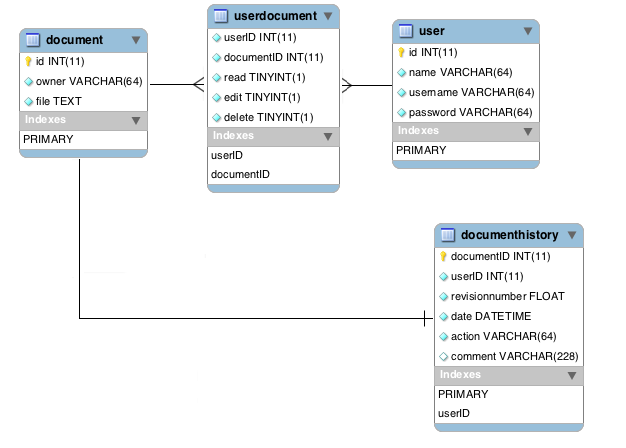
\includegraphics[width=300px]{images/ER-Diagram.png}
    	\caption{ER-Diagram}
	\end{figure}
	
\section{Slice of Pie user manual}
\label{sec-1}
\subsection{Starting the application}
\label{sec-1-1}
\subsubsection{Running the application from Visual Studio}
\label{sec-1-1-1}

    Before starting the application, you need to start Visual Studio with administration priviledges.
    The reason for this is that the application will need to create files and folders for the documents
    and in order to do so the program needs to be run with administrator priviledges which will give the 
    application write access.

    Since the web client runs in the browser, the browser needs to allow pop up windows for localhost.
    This can be done when the application is run for the first time.

    When starting the application, you need to set the WebClient project as startup project (if it's not
    already set), and then run the program (f5 for debug mode, ctrl + f5 for the release version).

    The web client will start up with your default internet browser. 
    When the main page has loaded, you are ready to use the application.
\subsubsection{Signing up}
\label{sec-1-1-2}

    As a first time user there won't be any user registered in the system, so the first time you need
    to do is to sign up to use the system.

    To sign up, click the ``Sign up'' button. This will open up a new window with the sign up form.

    Fill out the form and click the ``Sign up'' button. A message will appear to say if the signup
    was successfull or not.

    If the signup was successfull you are now registered in the system, and are ready to use it. 
    Close the sign up window and go back to the main window.
\subsubsection{Logging in}
\label{sec-1-1-3}

    On the main screen there are two text boxes at the top of the window named ``username'' and ``password''.
    Enter the newly created username and password into the boxes and click the ``Login'' button.
\subsection{Using the system}
\label{sec-1-2}

   After you have logged in, press the ``Get Files'' button on the left page of the window. 
   This will show you all the files that belong to the current user. Since you are a new user you don't 
   have any documents, so you should only see the root folder (the one with your username).
\subsubsection{Create a new document.}
\label{sec-1-2-1}

    To create a new document, click the ``New Document''. This will clear all text boxes, and you are ready
    to write a new document.

    Creating a new document doesn't save the document, so before you go too far you should save your document.
    Write a filename in the filename box, and click the ``Save Document'' button.
    If you wish to save the document in a sub folder, just write the: ``foldername/filename.html'' in the filebox.

    The system doesn't require that you save the document as a HTML file, but the system is built around it. Not 
    doing so won't make it able to add images to you document.
\subsubsection{Deleting a document}
\label{sec-1-2-2}

    Deleting a document is very simple.
    Select a document from the list on the left. Make sure that the filename of the file is entered into the 
    filename box (this can also be done manually). Delete the document by clicking the ``Delete Document'' button.
\subsubsection{Sharing a document}
\label{sec-1-2-3}

    Sharing a document is very simple as well.
    Open the document you wish to share. Enter the username of the user you wish to share the document with in
    the text box next to the ``Share Document'' button, and click the share document button.
\subsubsection{Showing a document}
\label{sec-1-2-4}

    Since the document is built around the HTML format, the text area can't show any images or text formatting.
    In order to see the document (with images, formatting etc) you need to open it in another page in the 
    browser.
    Select the document you wish to view and click the ``Show Document'' button. This will open a new window 
    with your document in parsed HTML.



\section{Revision Table}
\begin{table}[h]
\caption{Revision Table}
\begin{center}
\begin{tabular}{c|c|c|c}
\hline 
Revision & Changes & Section & Author \\ \hline 
21-11-12 & Created Vision & 1 & Bergar \\ 
21-11-12 & Created Use cases & 2 & Bergar \\
21-11-12 & Use case 1 and 2 & 2 & Filip \\
21-11-12 & Created Glossary & 3 & \\
21-11-12 & Created Supplementary Specifications & 4 & Bergar \\ 
21-11-12 & Created Domain Model diagram & 5 & Bergar and Filip \\
21-11-12 & Created Logical Architecture diagram & 6 & Bergar and Filip \\
\hline 
22-11-12 & System Sequence Diagram & 7 & Bergar \\
22-11-12 & Operation Contracts & 8 & Bergar \\
22-11-12 & Use cases 3, 4, 6 and 7 & 2 & Morten \\
22-11-12 & Use case diagram & 9 & Filip \\
\hline
23-11-12 & UML Package Diagram & 10 & Bergar \\
23-11-12 & UML Class Diagram & 11 & Bergar \\
\hline
27-11-12 & UML Communication Diagram & 12 & Morten \\
\hline
04-12-12 & Use case 10 & 2 & Bergar \\
04-12-12 & Update class diagram & 12 & Bergar \\
04-12-12 & Technical memo for file format & 13 & Bergar \\
04-12-12 & ER-Diagram & 14 & Bergar and Morten  \\
\hline
16-12-12 & Use case 4, 8 and 9 & 2 & Bergar \\
16-12-12 & Updated supplementary requirements & 4 & Bergar \\
16-12-12 & Updated use case diagram & 9 & Bergar \\
16-12-12 & Merging Technical memo & 13 & Bergar \\
16-12-12 & Updated class diagram & 11 & Bergar \\
16-12-12 & Application user manual & 16 & Bergar \\
\hline
\end{tabular} 
\end{center}
\end{table}
	
\end{document}